%
% lemniskate.tex
%
% (c) 2021 Prof Dr Andreas Müller, OST Ostschweizer Fachhochschule
%
\section{Lemniskatischer Sinus
\label{buch:elliptisch:section:lemniskate}}
\rhead{Lemniskatischer Sinus}
Historisch war der {\em lemniskatische Sinus} die erste ellptische
Funktion, die Gauss bereits als 19-jähriger untersucht, aber nicht 
veröffentlich hat.
In diesem Abschnitt soll die Verbindung zu den Jacobischen
elliptischen Funktionen hergestellt werden.

\subsection{Lemniskate
\label{buch:gemotrie:subsection:lemniskate}}
\begin{figure}
\centering
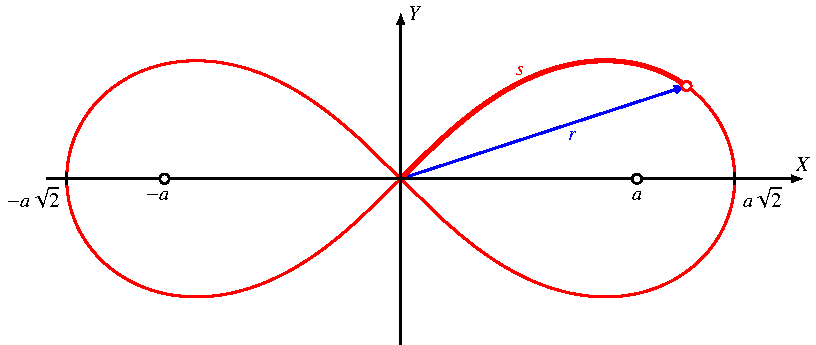
\includegraphics{chapters/110-elliptisch/images/lemniskate.pdf}
\caption{Bogenlänge und Radius der Lemniskate von Bernoulli.
\label{buch:elliptisch:fig:lemniskate}}
\end{figure}
Die Lemniskate von Bernoulli ist die Kurve vierten Grades mit der Gleichung
\begin{equation}
(X^2+Y^2)^2 = 2a^2(X^2-Y^2).
\label{buch:elliptisch:eqn:lemniskate}
\end{equation}
Sie ist in Abbildung~\ref{buch:elliptisch:fig:lemniskate}
dargestellt.
Die beiden Scheitel der Lemniskate befinden sich bei $X_s=\pm a\sqrt{2}$.
Dividiert man die Gleichung der Lemniskate durch $X_s^2=4a^4$ entsteht 
\begin{equation}
\biggl(
\biggl(\frac{X}{a\sqrt{2}}\biggr)^2
+
\biggl(\frac{Y}{a\sqrt{2}}\biggr)^2
\biggr)^2
=
2\frac{a^2}{2a^2}\biggl(
\biggl(\frac{X}{a\sqrt{2}}\biggr)^2
-
\biggl(\frac{Y}{a\sqrt{2}}\biggr)^2
\biggr).
\qquad
\Leftrightarrow
\qquad
(x^2+y^2)^2 = x^2-y^2,
\label{buch:elliptisch:eqn:lemniskatenormiert}
\end{equation}
wobei wir $x=X/a\sqrt{2}$ und $y=Y/a\sqrt{2}$ gesetzt haben.
In dieser Normierung liegen die Scheitel bei $\pm 1$.
Dies ist die Skalierung, die für die Definition des lemniskatischen
Sinus und Kosinus verwendet werden soll.

In Polarkoordinaten $x=r\cos\varphi$ und $y=r\sin\varphi$
gilt nach Einsetzen in \eqref{buch:elliptisch:eqn:lemniskatenormiert}
\begin{equation}
r^4
=
r^2(\cos^2\varphi-\sin^2\varphi)
=
r^2\cos2\varphi
\qquad\Rightarrow\qquad
r^2 = \cos 2\varphi
\label{buch:elliptisch:eqn:lemniskatepolar}
\end{equation}
als Darstellung der Lemniskate in Polardarstellung.
Sie gilt für Winkel $\varphi\in[-\frac{\pi}4,\frac{\pi}4]$ für das
rechte Blatt und $\varphi\in[\frac{3\pi}4,\frac{5\pi}4]$ für das linke
Blatt der Lemniskate.

\subsection{Bogenlänge}
Die Funktionen
\begin{equation}
x(r) = \frac{r}{\sqrt{2}}\sqrt{1+r^2},
\quad
y(r) = \frac{r}{\sqrt{2}}\sqrt{1-r^2}
\label{buch:geometrie:eqn:lemniskateparam}
\end{equation}
erfüllen
\begin{align*}
x(r)^2-y(r)^2
&=
\frac{r^2(1+r^2)}{2}-\frac{r^2(1-r^2)}{2}
\\
&
=
r^4
=
(x(r)^2 + y(r)^2)^2,
\end{align*}
sie stellen also eine Parametrisierung der Lemniskate dar.

Mit Hilfe der Parametrisierung~\eqref{buch:geometrie:eqn:lemniskateparam}
kann man die Länge $s$ des in Abbildung~\ref{buch:elliptisch:fig:lemniskate}
dargestellten Bogens der Lemniskate berechnen.
Dazu benötigt man die Ableitungen nach $r$, die man mit der Produkt- und
Kettenregel berechnen kann:
\begin{align*}
\dot{x}(r)
&=
\frac{\sqrt{1+r^2}}{\sqrt{2}}
+
\frac{r^2}{\sqrt{2}\sqrt{1+r^2}}
&&\Rightarrow&
\dot{x}(r)^2
&=
\frac{1+r^2}{2} +r^2 + \frac{r^4}{2(1+r^2)}
\\
\dot{y}(r)
&=
\frac{\sqrt{1-r^2}}{\sqrt{2}}
-
\frac{r^2}{\sqrt{2}\sqrt{1-r^2}}
&&\Rightarrow&
\dot{y}(r)^2
&=
\frac{1-r^2}{2} -r^2 + \frac{r^4}{2(1-r^2)}
\end{align*}
Die Summe der Quadrate ist
\begin{align*}
\dot{x}(r)^2 + \dot{y}(r)^2
&=
1 + r^4\frac{1-r^2+1+r^2}{2(1+r^2)(1-r^2)}
=
1+r^4\frac{2}{2(1-r^4)}
=
\frac{1-r^4+r^4}{1-r^4}
=
\frac1{1-r^4}.
\end{align*}
Durch Einsetzen in das Integral für die Bogenlänge bekommt man
\begin{equation}
s(r)
=
\int_0^r
\frac{1}{\sqrt{1-t^4}}\,dt.
\label{buch:elliptisch:eqn:lemniskatebogenlaenge}
\end{equation}

%
% Als elliptisches Integral
%
\subsection{Darstellung als elliptisches Integral}
Das unvollständige elliptische Integral erster Art mit Parameter
$k^2=-1$ oder $k=i$ ist
\[
K(r,i)
=
\int_0^x \frac{dt}{\sqrt{(1-t^2)(1-i^2 t^2)}}
=
\int_0^x \frac{dt}{\sqrt{(1-t^2)(1-(-1)t^2)}}
=
\int_0^x \frac{dt}{\sqrt{1-t^4}}
=
s(r).
\]
Der lemniskatische Sinus ist also eine Umkehrfunktion des
elliptischen Integrals erster Art für den speziellen Wert $i$ des
Parameters $k$.

Die Länge des rechten Blattes der Lemniskate wird mit $\varpi$ bezeichnet
und hat den numerischen Wert
\[
\varpi
=
2\int_0^1\sqrt{\frac{1}{1-t^4}}\,dt
=
2.6220575542.
\]
$\varpi$ ist auch als die {\em lemniskatische Konstante} bekannt.
\index{lemniskatische Konstante}%
Der Lemniskatenbogen zwischen dem Nullpunkt und $(1,0)$ hat die Länge
$\varpi/2$.

%
%  Bogenlängenparametrisierung
%
\subsection{Bogenlängenparametrisierung}
Die Lemniskate mit der Gleichung
\[
(X^2+X^2)^2=2(X^2-X^2)
\]
(der Fall $a=1$ in \eqref{buch:elliptisch:eqn:lemniskate})
kann mit Jacobischen elliptischen Funktionen
parametrisiert werden.
Dazu schreibt man
\[
\left.
\begin{aligned}
X(t)
&=
\sqrt{2}\operatorname{cn}(t,k) \operatorname{dn}(t,k)
\\
Y(t)
&=
\phantom{\sqrt{2}}
\operatorname{cn}(t,k) \operatorname{sn}(t,k)
\end{aligned}
\quad\right\}
\qquad\text{mit $k=\displaystyle\frac{1}{\sqrt{2}}$}
\]
und berechnet die beiden Seiten der definierenden Gleichung der
Lemniskate.
Zunächst ist
\begin{align*}
X(t)^2
&=
2\operatorname{cn}(t,k)^2
\operatorname{dn}(t,k)^2
\\
Y(t)^2
&=
\operatorname{cn}(t,k)^2
\operatorname{sn}(t,k)^2
\\
X(t)^2+Y(t)^2
&=
2\operatorname{cn}(t,k)^2
\bigl(
\underbrace{
\operatorname{dn}(t,k)^2
+{\textstyle\frac12}
\operatorname{sn}(t,k)^2
}_{\displaystyle =1}
\bigr)
%\\
%&
=
2\operatorname{cn}(t,k)^2
\\
X(t)^2-Y(t)^2
&=
\operatorname{cn}(t,k)^2
\bigl(
2\operatorname{dn}(t,k)^2 - \operatorname{sn}(t,k)^2
\bigr)
\\
&=
\operatorname{cn}(t,k)^2
\bigl(
2\bigl({\textstyle\frac12}+{\textstyle\frac12}\operatorname{cn}(t,k)^2\bigr)
-
\bigl(1-\operatorname{cn}(t,k)^2\bigr)
\bigr)
\\
&=
2\operatorname{cn}(t,k)^4
\\
\Rightarrow\qquad
(X(t)^2+Y(t)^2)^2
&=
4\operatorname{cn}(t,k)^4
=
2(X(t)^2-Y(t)^2).
\end{align*}
Wir zeigen jetzt, dass dies tatsächlich eine Bogenlängenparametrisierung
der Lemniskate ist.
Dazu berechnen wir die Ableitungen
\begin{align*}
\dot{X}(t)
&=
\sqrt{2}\operatorname{cn}'(t,k)\operatorname{dn}(t,k)
+
\sqrt{2}\operatorname{cn}(t,k)\operatorname{dn}'(t,k)
\\
&=
-\sqrt{2}\operatorname{sn}(t,k)\operatorname{dn}(t,k)^2
-\frac12\sqrt{2}\operatorname{sn}(t,k)\operatorname{cn}(t,k)^2
\\
&=
-\sqrt{2}\operatorname{sn}(t,k)\bigl(
1-{\textstyle\frac12}\operatorname{sn}(t,k)^2
+{\textstyle\frac12}-{\textstyle\frac12}\operatorname{sn}(u,t)^2
\bigr)
\\
&=
\sqrt{2}\operatorname{sn}(t,k)
\bigl(
{\textstyle \frac32}-\operatorname{sn}(t,k)^2
\bigr)
\\
\dot{X}(t)^2
&=
2\operatorname{sn}(t,k)^2
\bigl(
{\textstyle \frac32}-\operatorname{sn}(t,k)^2
\bigr)^2
\\
&=
{\textstyle\frac{9}{2}}\operatorname{sn}(t,k)^2
-
6\operatorname{sn}(t,k)^4
+2\operatorname{sn}(t,k)^6
\\
\dot{Y}(t)
&=
\operatorname{cn}'(t,k)\operatorname{sn}(t,k)
+
\operatorname{cn}(t,k)\operatorname{sn}'(t,k)
\\
&=
-\operatorname{sn}(t,k)^2
\operatorname{dn}(t,k)
+\operatorname{cn}(t,k)^2
\operatorname{dn}(t,k)
\\
&=
\operatorname{dn}(t,k)\bigl(1-2\operatorname{sn}(t,k)^2\bigr)
\\
\dot{Y}(t)^2
&=
\bigl(1-{\textstyle\frac12}\operatorname{sn}(t,k)^2\bigr)
\bigl(1-2\operatorname|{sn}(t,k)^2\bigr)^2
\\
&=
1-{\textstyle\frac{9}{2}}\operatorname{sn}(t,k)^2
+6\operatorname{sn}(t,k)^4
-2\operatorname{sn}(t,k)^6
\\
\dot{X}(t)^2 + \dot{Y}(t)^2
&=
1.
\end{align*}
Dies bedeutet, dass die Bogenlänge zwischen den Parameterwerten $0$ und $s$
\[
\int_0^s
\sqrt{\dot{X}(t)^2 + \dot{Y}(t)^2}
\,dt
=
\int_0^s\,dt
=
s,
\]
der Parameter $t$ ist also ein Bogenlängenparameter.

Die mit dem Faktor $1/\sqrt{2}$ skalierte Standard-Lemniskate mit der
Gleichung
\[
(x^2+y^2)^2 = x^2-y^2
\]
hat daher eine Bogenlängenparametrisierung mit
\begin{equation}
\begin{aligned}
x(t)
&=
\phantom{\frac{1}{\sqrt{2}}}
\operatorname{cn}(\sqrt{2}t,k)\operatorname{dn}(\sqrt{2}t,k)
\\
y(t)
&=
\frac{1}{\sqrt{2}}\operatorname{cn}(\sqrt{2}t,k)\operatorname{sn}(\sqrt{2}t,k)
\end{aligned}
\label{buch:elliptisch:lemniskate:bogenlaenge}
\end{equation}

\subsection{Der lemniskatische Sinus und Kosinus}
Der Sinus Berechnet die Gegenkathete zu einer gegebenen Bogenlänge des
Kreises, er ist die Umkehrfunktion der Funktion, die der Gegenkathete
die Bogenlänge zuordnet.

Daher ist es naheliegend, die Umkehrfunktion von $s(r)$ in 
\eqref{buch:elliptisch:eqn:lemniskatebogenlaenge}
den {\em lemniskatischen Sinus} zu nennen mit der Bezeichnung
$r=\operatorname{sl} s$.

Der Kosinus ist der Sinus des komplementären Winkels.
Auch für die lemniskatische Bogenlänge $s(r)$ lässt sich eine
komplementäre Bogenlänge definieren, nämlich die Bogenlänge zwischen
dem Punkt $(x(r), y(r))$ und $(1,0)$.

Da die Parametrisierung~\eqref{buch:elliptisch:lemniskate:bogenlaenge}
eine Bogenlängenparametrisierung ist, darf man $t=s$ schreiben.
Dann kann man aber auch $r(s)$ daraus berechnen,
es ist
\[
r(s)^2
=
x(s)^2 + y(s)^2
=
\operatorname{cn}(s\sqrt{2},k)^2
\qquad\Rightarrow\qquad
r(s)
=
\operatorname{cn}(s\sqrt{2},k)
\]

\begin{figure}
\centering
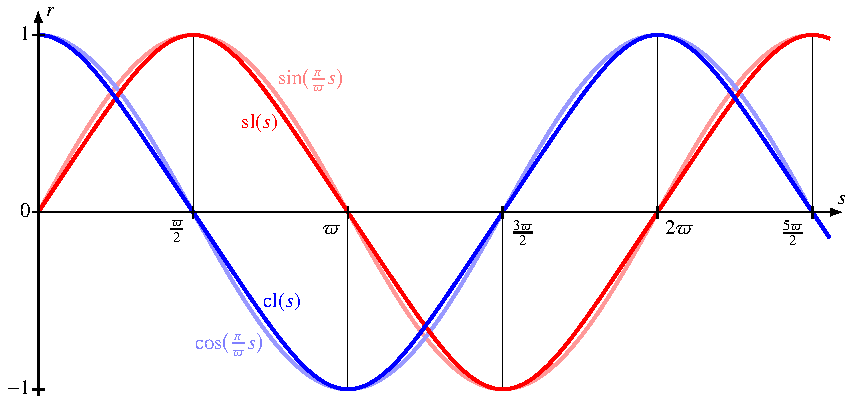
\includegraphics[width=\textwidth]{chapters/110-elliptisch/images/slcl.pdf}
\caption{
Lemniskatischer Sinus und Kosinus sowie Sinus und Kosinus
mit derart skaliertem Argument, dass die Funktionen die gleichen Nullstellen
haben.
\label{buch:elliptisch:figure:slcl}}
\end{figure}
